\documentclass[tikz,border=2pt]{standalone}
\usepackage{amsmath,amssymb}
\usepackage{pgfplots}
\pgfplotsset{compat=1.18}
\usetikzlibrary{arrows.meta}
\begin{document}
% Exponential loss with rate lambda = 1/2: the area under the survivor function e^{-t/2} beyond d = 2 equals
% pi_X(2) = e^{-lambda d}/lambda = 2e^{-1} ~ 0.74; the transform pi_X(d) = 2e^{-d/2} starts at E[X] = 2 and decreases convexly.
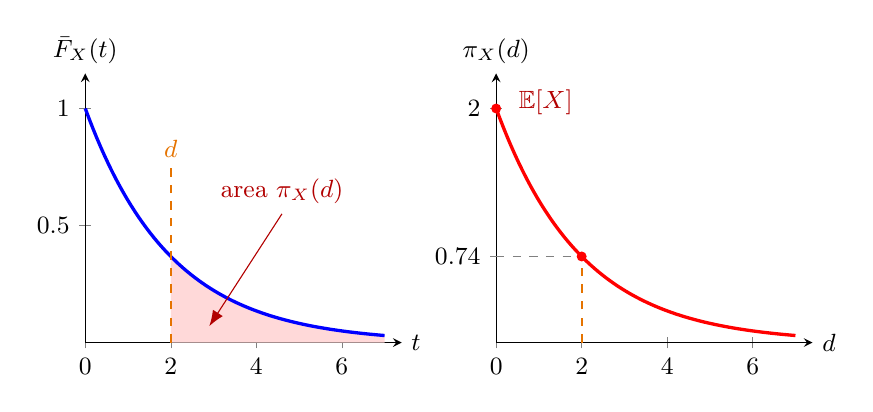
\begin{tikzpicture}[font=\small, >={Latex[length=2mm]}]
  \begin{axis}[name=left,
    axis lines=left, xmin=0, xmax=7.4, ymin=0, ymax=1.15,
    xtick={0,2,4,6}, ytick={0.5,1},
    xlabel={$t$}, ylabel={$\bar F_X(t)$},
    xlabel style={at={(axis description cs:1,0)}, anchor=west},
    ylabel style={rotate=-90, at={(axis description cs:0,1)}, anchor=south},
    width=5.6cm, height=5cm, clip=false]
    \addplot[fill=red!15, draw=none, domain=2:7, samples=60] {exp(-x/2)} \closedcycle;
    \addplot[blue, very thick, domain=0:7, samples=80] {exp(-x/2)};
    \draw[orange!90!black, thick, dashed] (axis cs:2,0) -- (axis cs:2,0.75);
    \node[orange!90!black, anchor=south] at (axis cs:2,0.75) {$d$};
    \draw[red!70!black, ->] (axis cs:4.6,0.55) -- (axis cs:2.9,0.07);
    \node[red!70!black, anchor=south] at (axis cs:4.6,0.55) {area $\pi_X(d)$};
  \end{axis}
  \begin{axis}[at={(left.east)}, anchor=west, xshift=1.2cm,
    axis lines=left, xmin=0, xmax=7.4, ymin=0, ymax=2.3,
    xtick={0,2,4,6}, ytick={0.74,2}, yticklabels={$0.74$,$2$},
    xlabel={$d$}, ylabel={$\pi_X(d)$},
    xlabel style={at={(axis description cs:1,0)}, anchor=west},
    ylabel style={rotate=-90, at={(axis description cs:0,1)}, anchor=south},
    width=5.6cm, height=5cm, clip=false]
    \addplot[red, very thick, domain=0:7, samples=80] {2*exp(-x/2)};
    \draw[orange!90!black, thick, dashed] (axis cs:2,0) -- (axis cs:2,0.7358);
    \draw[gray, thin, dashed] (axis cs:0,0.7358) -- (axis cs:2,0.7358);
    \fill[red] (axis cs:2,0.7358) circle (1.8pt);
    \fill[red] (axis cs:0,2) circle (1.8pt);
    \node[red!70!black, anchor=west] at (axis cs:0.3,2.05) {$\mathbb{E}[X]$};
  \end{axis}
\end{tikzpicture}
\end{document}
